\documentclass[]{article}
\usepackage[a4paper, total={6in, 10in}]{geometry}
\usepackage{hyperref}
\usepackage{amsmath}
\usepackage{graphicx}
\usepackage[outdir=./]{epstopdf}
\usepackage{booktabs}
\usepackage{float}

\setlength{\parindent}{0em}
\setlength{\parskip}{1em}

%opening
\title{SSY 230, System Identification\\
	Project 1: Estimating functions from noisy data}
\author{Yuxuan Xia\\ \href{mailto:yuxuan.xia@chalmers.se}{yuxuan.xia@chalmers.se}}

\begin{document}

\maketitle

\section{Linear regression functions}

\subsection{Estimation parameter validation}

\subsection{Regularization verification}

Given a regressor matrix $\mathbf{x}$ and an output matrix $\mathbf{y}$, the linear least squares estimate with L2-Regularization can be obtained by minimizing the sum of squared residuals,
\begin{equation}{\label{LSestimator}}
\hat{\theta} = \arg\min\limits_{\theta}(\mathbf{y}-\mathbf{x}\theta)^T(\mathbf{y}-\mathbf{x}\theta)+\lambda\theta^T\theta.
\end{equation}
The estimate $\hat{\theta}$ can be found by setting the derivative of (\ref{LSestimator}) w.r.t. $\theta$ to zero,
\begin{subequations}\label{LSderivative}
		\begin{align}
		\frac{d}{d\theta}\left((\mathbf{y}-\mathbf{x}\theta)^T(\mathbf{y}-\mathbf{x}\theta)+\lambda\theta^T\theta \right) &= 0,\\
		-\mathbf{x}^T\mathbf{y}+\mathbf{x}^T\mathbf{x}\theta+\lambda\theta &=0,\\
		(\mathbf{x}^T\mathbf{x}+\lambda\mathbf{I})^{-1}\mathbf{x}^T\mathbf{y} &=\hat{\theta}.
		\end{align}
\end{subequations}
It is easy to verify that, when $\lambda=0$, $\hat{\theta}$ is equal to the linear least squares estimate without regularization, i.e.,
\begin{equation}
\hat{\theta} = (\mathbf{x}^T\mathbf{x})^{-1}\mathbf{x}^T\mathbf{y},
\end{equation}
and that, when $\lambda\rightarrow +\infty$, $\hat{\theta}\rightarrow \mathbf{0}$.


\subsection{Polynomial fitting validation}

\subsection{One dimensional model plotting}
\begin{figure}[H]
	\caption{Estimated function using linear regression.}
	\centering
	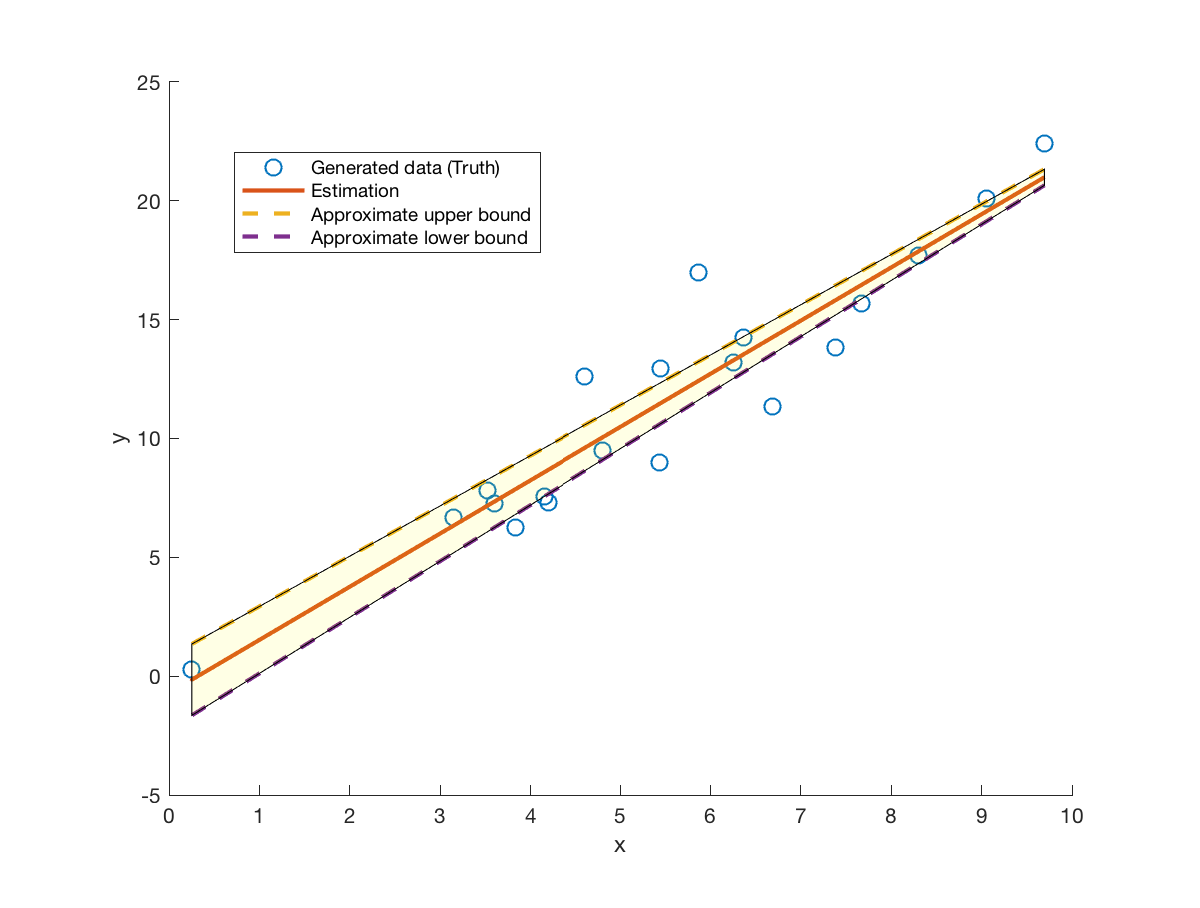
\includegraphics[width=0.8\textwidth]{project1e.eps}
\end{figure}

\section{KNN-regression functions}

\subsection{KNN v.s. Linear regression}
\begin{figure}[H]
	\caption{Estimated functions using linear regression and KNN (K=3).}
	\centering
	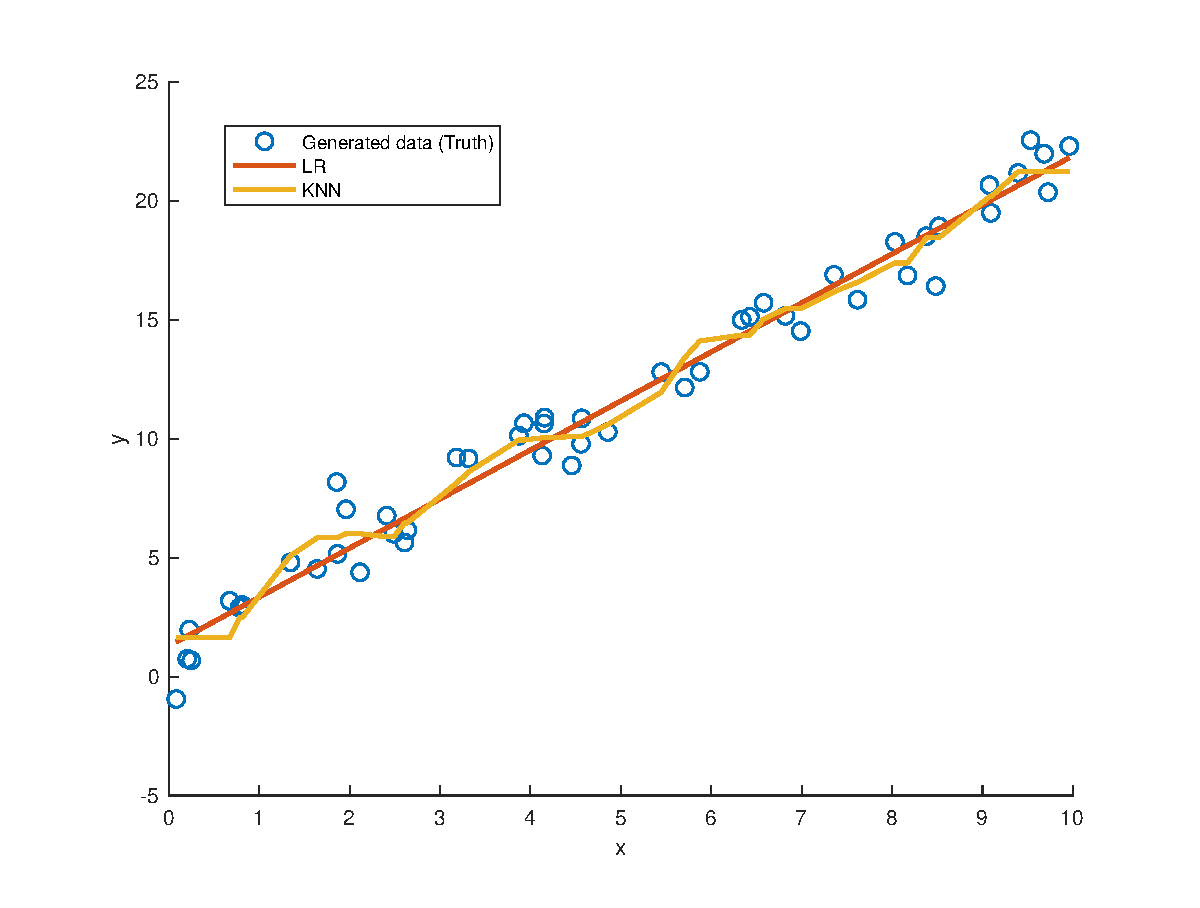
\includegraphics[width=0.8\textwidth]{project2b}
\end{figure}

\section{Estimating one dimensional functions}

\subsection{Linear data}

\subsubsection{Linear regression model (constant + linear term)}
\begin{table}[H]
	\centering
	\caption{Estimation results of a linear regression model with only constant and linear terms.}
	\label{tab:linear}
	\begin{tabular}{@{}ccc@{}}
		\toprule
		Generated data size (N) & Constant estimation & Linear term estimation \\ \midrule
		N=10        & 1.74                & 0.45                   \\
		N=100       & 1.34                & 0.53                   \\
		N=1000      & 1.63                & 0.48                   \\
		N=10000     & 1.47                & 0.50                   \\ \bottomrule
	\end{tabular}
\end{table}

As suggested by the results shown in Table \ref{tab:linear}, the estimates converge to the true function $\mathbf{y}=1.5+0.5\mathbf{x}$ when the number of data goes to infinity. 

\subsubsection{Linear regression model (5th order polynomial)}
\begin{figure}[H]
	\caption{Model quality (mean square error) v.s. Number of data}
	\centering
	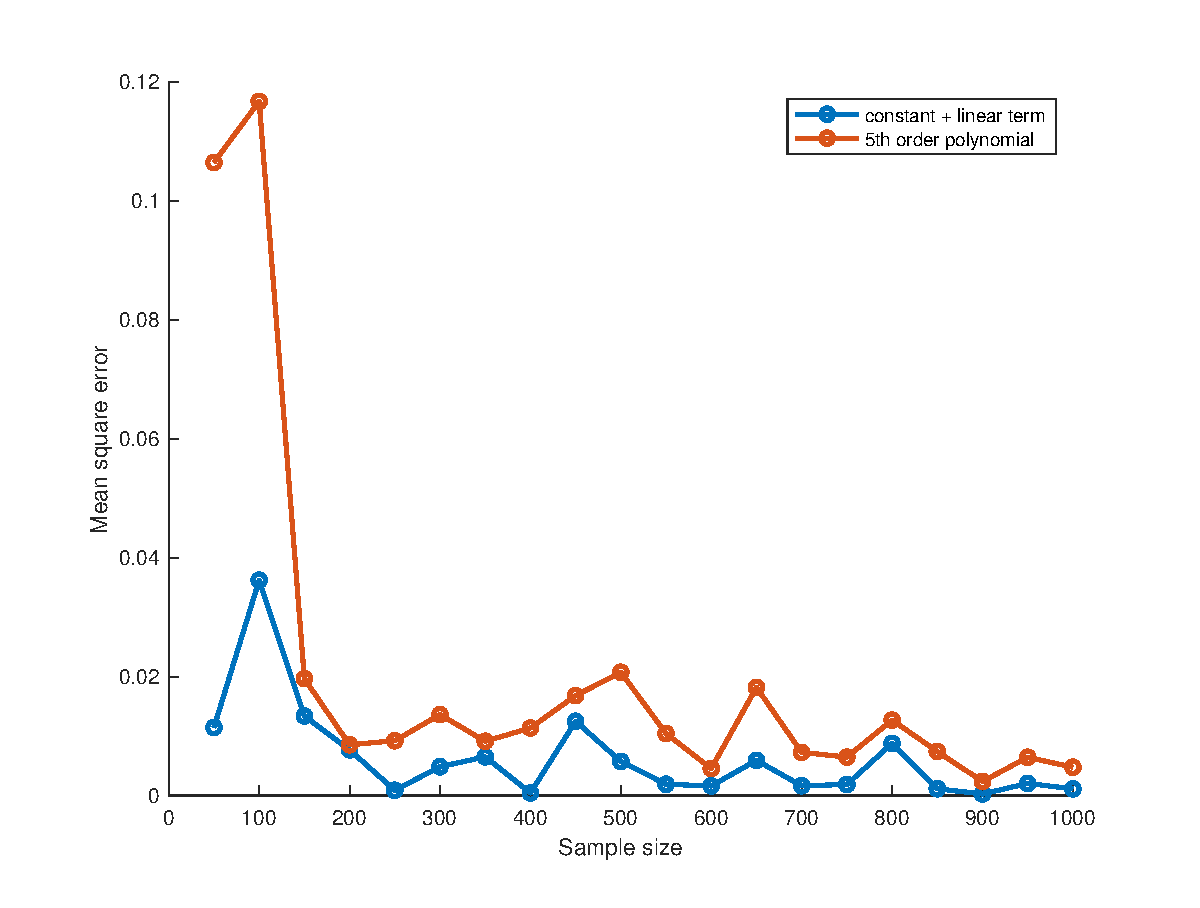
\includegraphics[width=0.8\textwidth]{project3c}
\end{figure}

The linear regression model with only constant and linear terms has better model quality in terms of mean square error than the linear regression model with polynomial terms. The difference between these two models, in general, becomes smaller as the number of data increases. This is because that the frequency of overfitting decreases as the data size increases. 


\subsubsection{Parameter variance validation via Monte Carlo simulation}
\begin{figure}[H]
	\caption{Histogram of parameter estimates using 1000 generated data over 1000 Monte Carlo trials.}
	\centering
	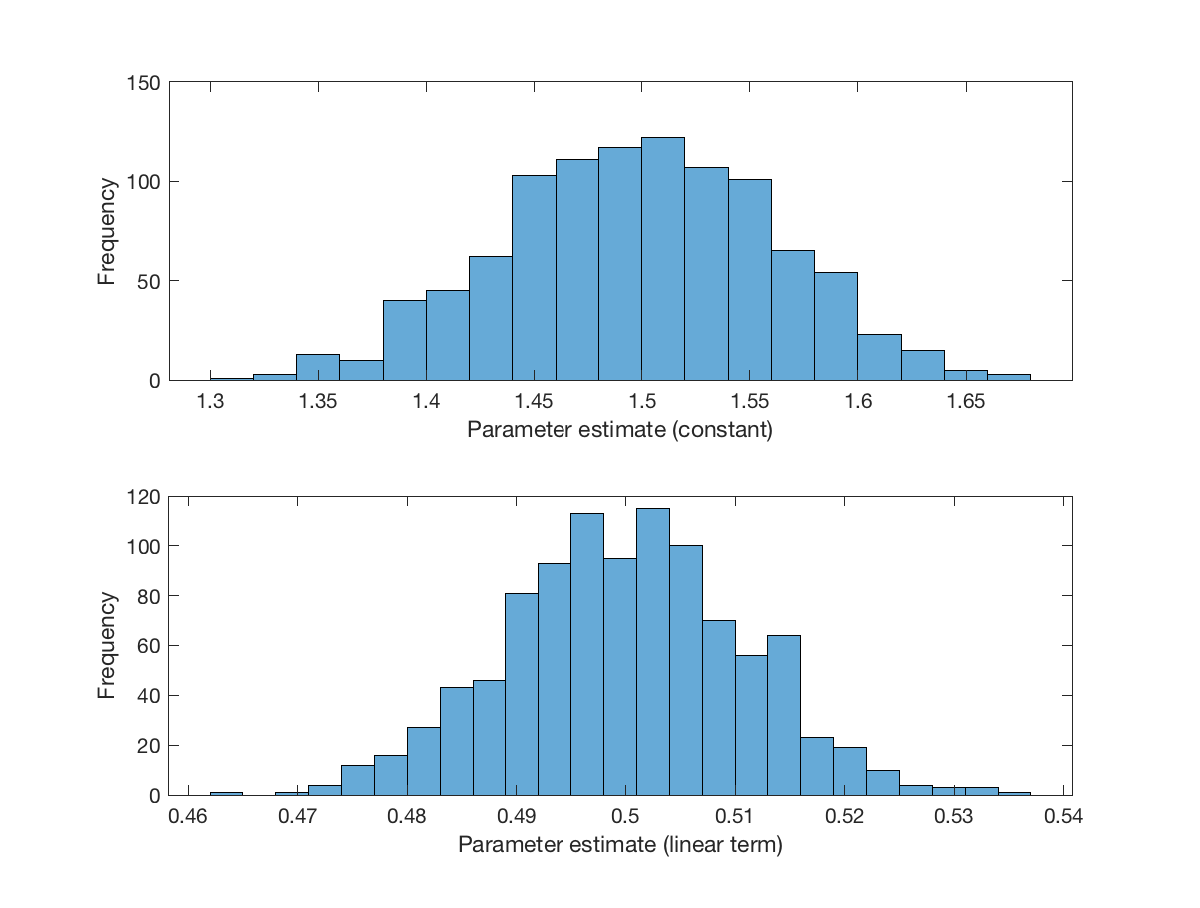
\includegraphics[width=0.8\textwidth]{project3c2}
\end{figure}

\subsubsection{KNN models}
\begin{figure}[H]
	\caption{Model quality (mean square error) of KNN model v.s. number of neighbors and number of data. Noise variance is 1.}
	\label{fig:KNNnumberofdata}
	\centering
	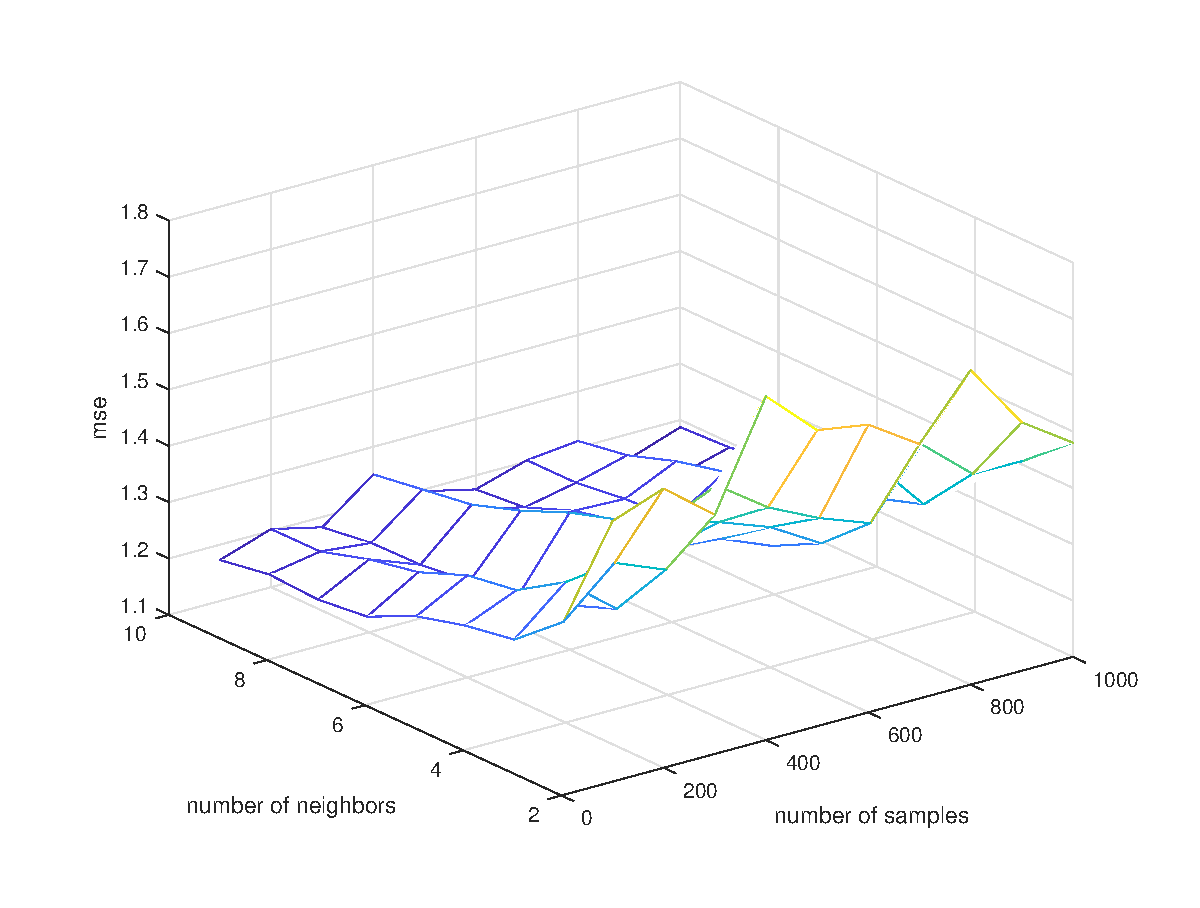
\includegraphics[width=0.8\textwidth]{project3d1}
\end{figure}

\begin{figure}[H]
	\caption{Model quality (mean square error) of KNN model v.s. number of neighbors and noise variance. Data size is 1000.}
	\label{fig:KNNnoisevariance}
	\centering
	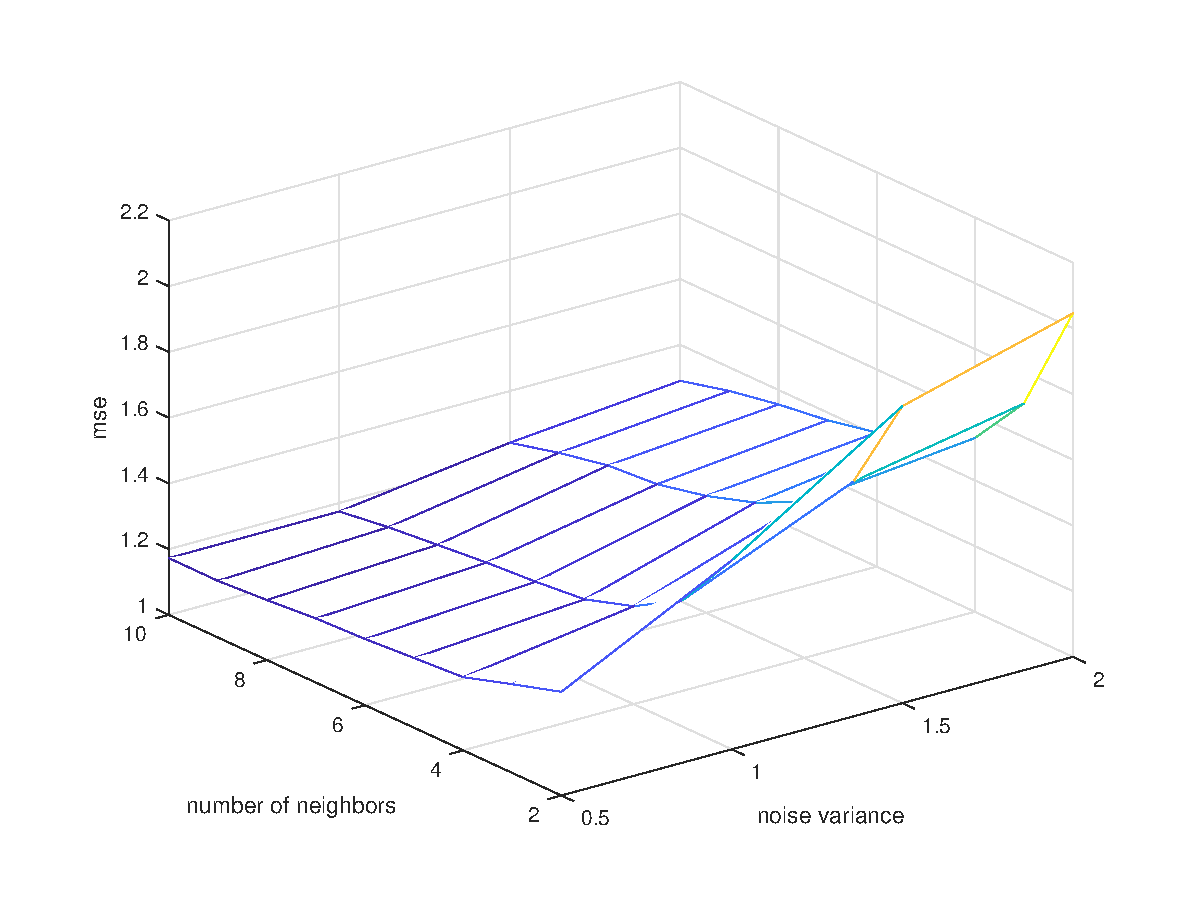
\includegraphics[width=0.8\textwidth]{project3d2}
\end{figure}

It can be seen from the results that the model quality of KNN model depends on both the data size and the noise variance. The results also suggest that a heuristically optimal number $K$ of nearest neighbors can be found based on the variance-bias trade-off. A general rule is that the larger the noise variance and the larger the data size, the more the number of neighbors we should choose.

\subsection{Polynomial  data}

\subsubsection{Linear regression model (constant + linear term)}

When we regress non-linear data on linear regressors, the model does not converge to the correct function and the parameter uncertainty goes to zero when the number of data goes to infinity. Recall the expression for parameter estimation variance,
\begin{equation}
\text{var}(\hat{\theta}) = (\mathbf{x}^T\mathbf{x})^{-1}\sigma^2,
\end{equation}
where $\sigma^2$ is the noise variance. It can be found that the parameter uncertainty depends on $(\mathbf{x}^T\mathbf{x})^{-1}$, which further depends on the dimension of $\mathbf{x}$, i.e., the data size. The larger the data size, the smaller $(\mathbf{x}^T\mathbf{x})^{-1}$ and the smaller the parameter uncertainty. 

\subsubsection{Linear regression model (polynomial + regularization)}
\begin{figure}[H]
	\caption{Model quality (mean square error) v.s. Polynomial degree.}
	\label{fig:5thorderpolynomial}
	\centering
	\includegraphics[width=0.8\textwidth]{project32b}
\end{figure}

\begin{figure}[H]
	\caption{Model quality (mean square error) v.s. Regularization term.}
	\label{fig:regularization}
	\centering
	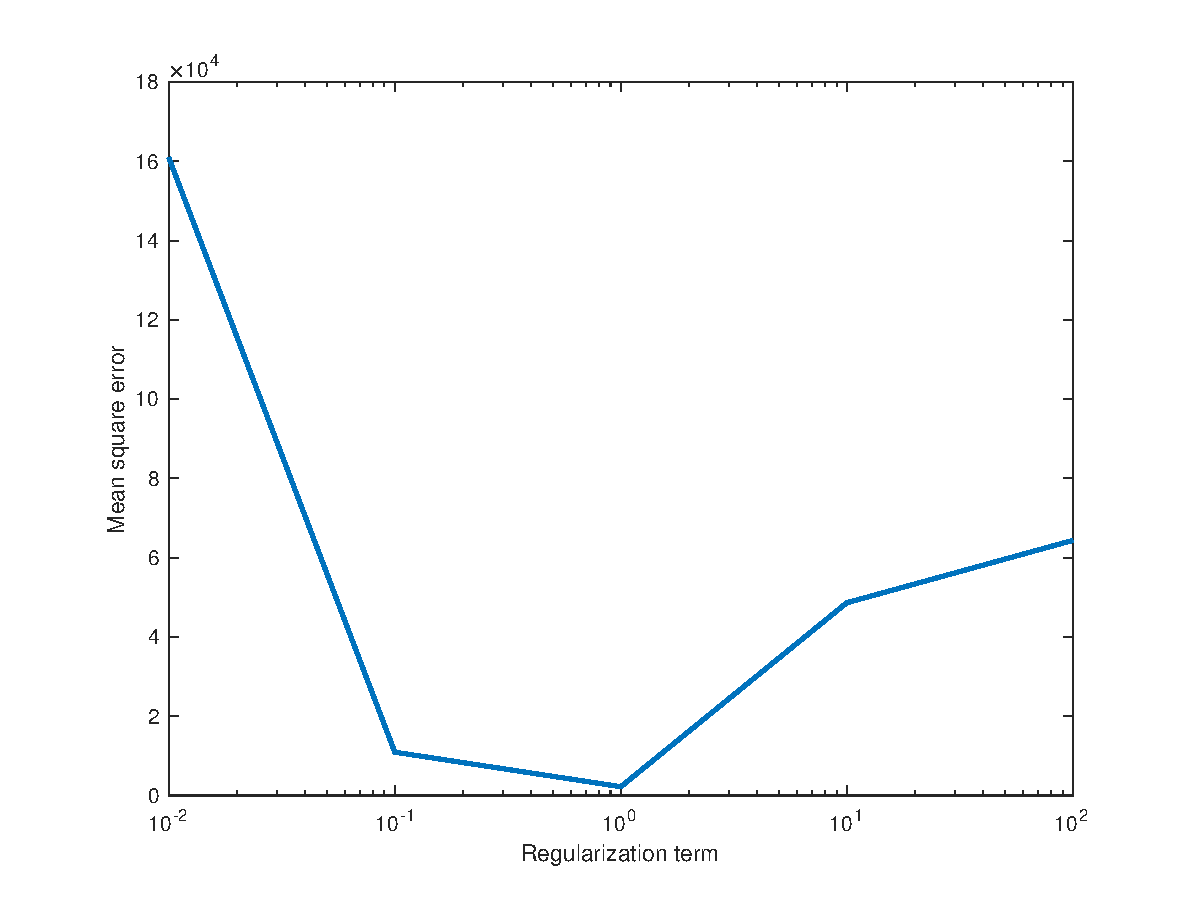
\includegraphics[width=0.8\textwidth]{project32b2}
\end{figure}

As can be seen from Figure. \ref{fig:5thorderpolynomial}, the best result (using 1000 generated data) is obtained when using a polynomial model with degree 4. When using a linear regressor with 10th order polynomial on a small data size, e.g., 15, the estimation does not fit the model due to overfitting. As shown in Figure. \ref{fig:regularization}, the estimation error can be reduced by adding regularization term; however, the size of the regularization term that gives the best model quality depends on the data.

\subsubsection{Regress unsymmetrical data using linear regression}
\begin{figure}[H]
	\caption{Regressing unsymmetrical data on a linear regressor (constant + linear term).}
	\label{fig:unsymmetrical}
	\centering
	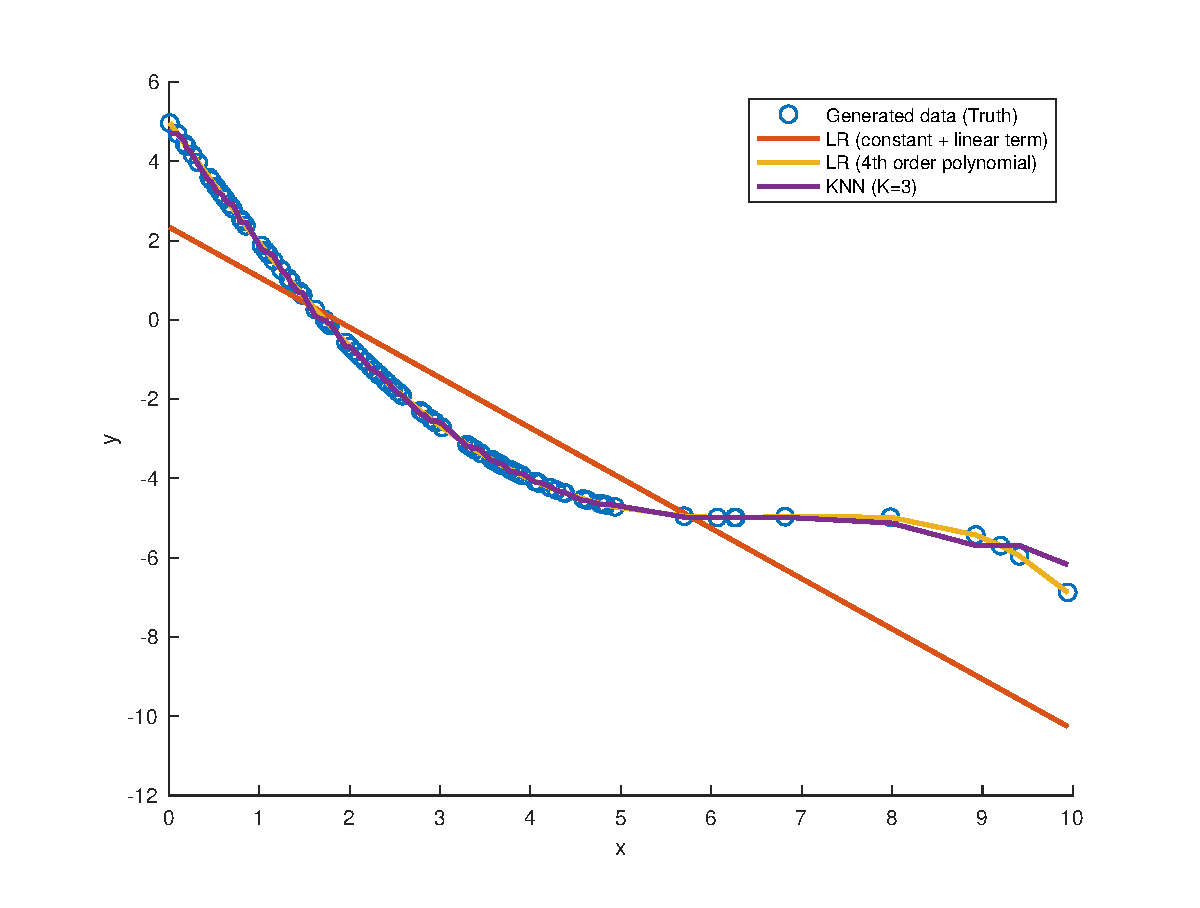
\includegraphics[width=0.8\textwidth]{project32c}
\end{figure}

As can be seen from Figure. \ref{fig:unsymmetrical}, the estimation does not fit the last part of the data due to non-linearity. In order to solve this problem, we can either increase the polynomial degree of the linear regression model we use or use a KNN model instead.

\subsubsection{Regress unsymmetrical data using KNN}
\begin{figure}[H]
	\caption{Regressing unsymmetrical data on a KNN. Noise variance is 1.}
	\label{fig:unsymmetricalKNN1}
	\centering
	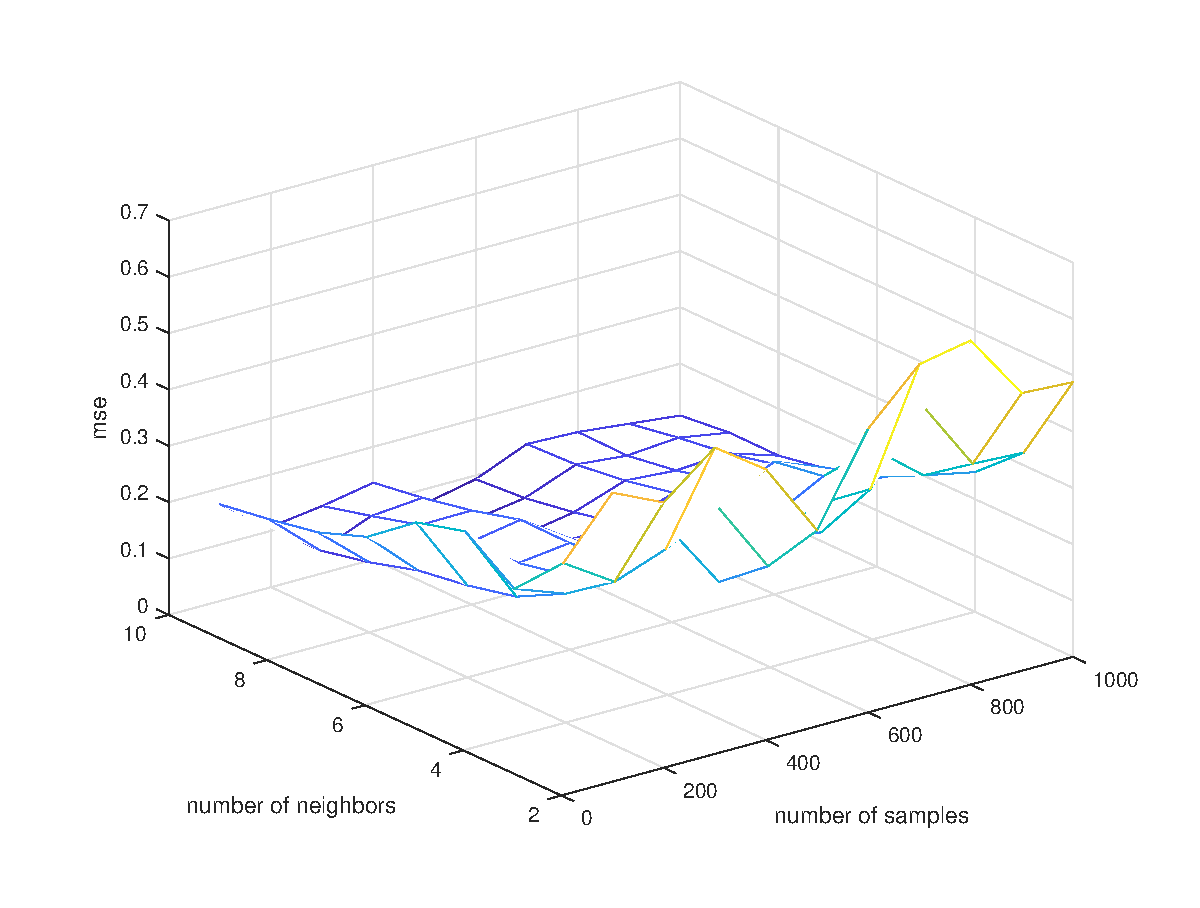
\includegraphics[width=0.8\textwidth]{project32d1}
\end{figure}

\begin{figure}[H]
	\caption{Regressing unsymmetrical data on a KNN. Data size is 1000.}
	\label{fig:unsymmetricalKNN2}
	\centering
	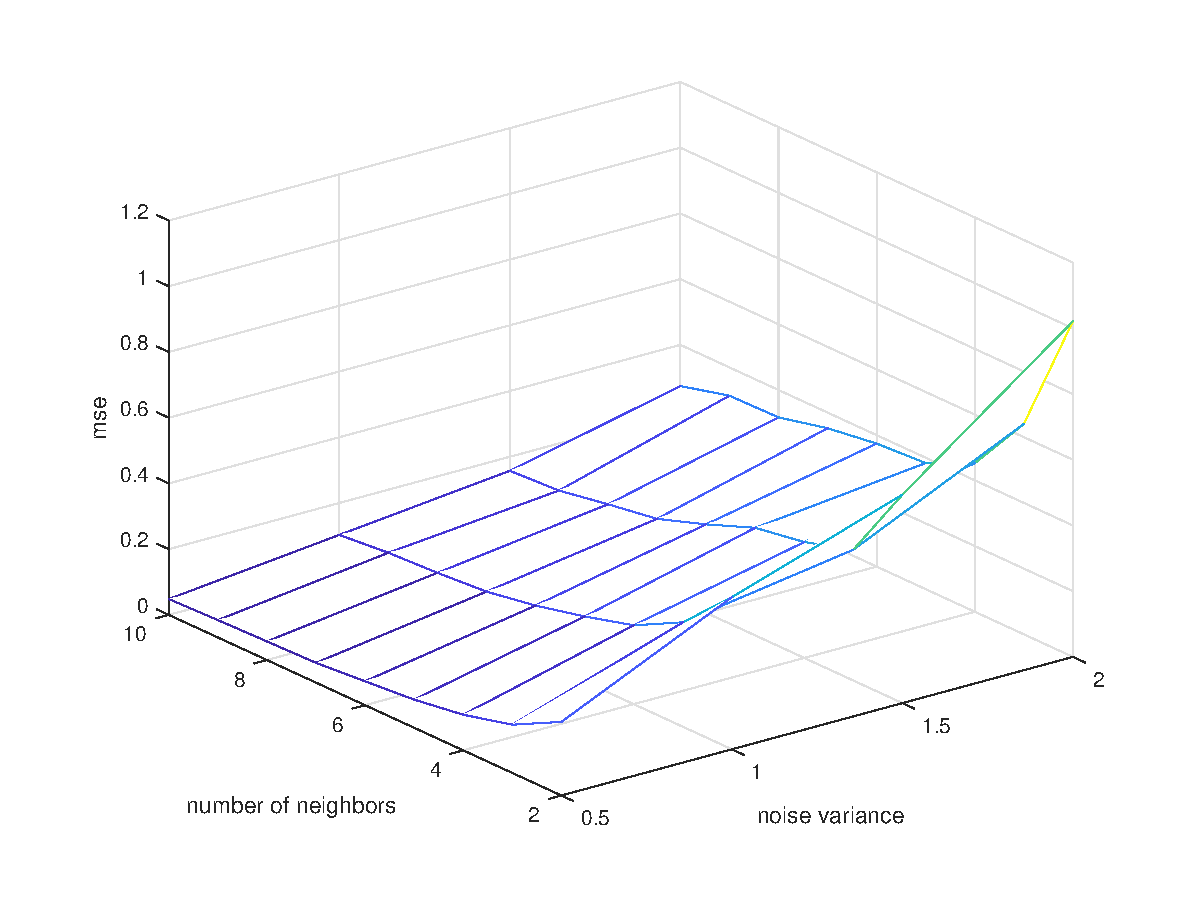
\includegraphics[width=0.8\textwidth]{project32d2}
\end{figure}

Figure. \ref{fig:unsymmetricalKNN1} shows how the model quality of KNN model varies with the number of neighbors and the number of data with fixed noise variance, and Figure. \ref{fig:unsymmetricalKNN2} shows how the model quality of KNN model varies with the number of neighbors and the number of data with fixed data size. A heuristically optimal number $K$ of nearest neighbors can be found based on the variance-bias trade-off.

\subsection{Chirp data}

\subsubsection{Influences of data size and noise level on polynomial model}

Empirical results show that better higher order model can be obtained by increasing the data size and decreasing the noise level. The ``best'' polynomial degree depends on the data since it is scholastically generated. When the data size is small and the noise level is high, overfitting is likely to happen because the model is working too hard to find patterns in the training data which are just cause by random chance. Hence, increasing the data size and lowering the noise level help reduce the chance of overfitting, which further provides a better estimation.

\subsubsection{High-degree polynomial with regularization v.s. Low-degree polynomial without regularization}

Generally speaking, if the degree of a polynomial model is too low to fit the data well, we then should choose a higher degree to have smaller estimation bias. The increased estimation variance can be reduced by regularization. By applying regularization, i.e., shrinking the estimated parameters, we can often substantially reduce the variance at the cost of a negligible increase in bias. 

\subsubsection{Linear regression v.s. KNN}

We have tested a linear regression model with polynomial degree two to ten and a KNN model with number of neighbors two to ten on generated data with size 50 and 1000 respectively. When the data size is small, the best performance of KNN is achieved by choosing the number of neighbors $K=2$. In this case, it is hard to say that KNN is better than linear regression. The specific comparison result depends on the polynomial degree of the linear regression, the randomly generated data and the noise level. However, when the data size is large, KNN outperforms linear regression with various degrees. In this case, the mean square error of the estimation result obtained using KNN is orders of magnitude less than the one using linear regression. 


\textbf{Analysis}: linear regression is an example of a parametric approach because it assumes a linear functional form for $f(\mathbf{x})$. Because the chirp data is highly non-linear, the resulting model after linear regression will provide a poor fit to the data. The non-linearity of the chirp data can be verified by finding the Taylor series of $\sin(\mathbf{x}^2)$, which has polynomial order towards infinity. As for the KNN model, a non-parametric regression approach, no explicit form for $f(\mathbf{x})$ is assumed, thus providing a more flexible estimation. 


\section{Estimating two and high dimensional functions}

\subsection{Two dimensional data}

The model quality can still be measured by calculating the  mean square error.

\subsubsection{Linear regression model}
\begin{figure}[H]
	\caption{Regressing twoDimData1 on a linear regression model}
	\label{fig:twodimData1}
	\centering
	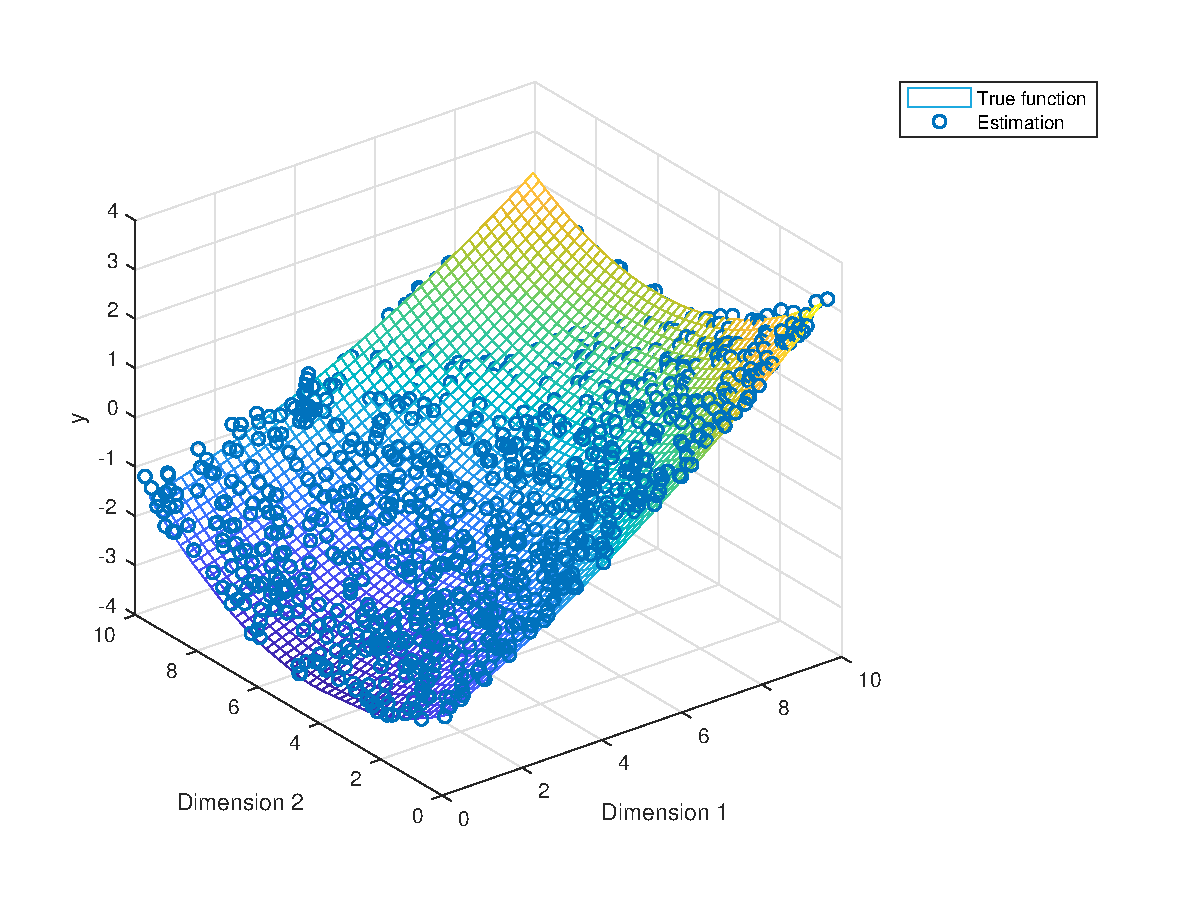
\includegraphics[width=0.8\textwidth]{project41c1}
\end{figure}

\begin{figure}[H]
	\caption{Regressing twoDimData2 on a linear regression model}
	\label{fig:twodimData2}
	\centering
	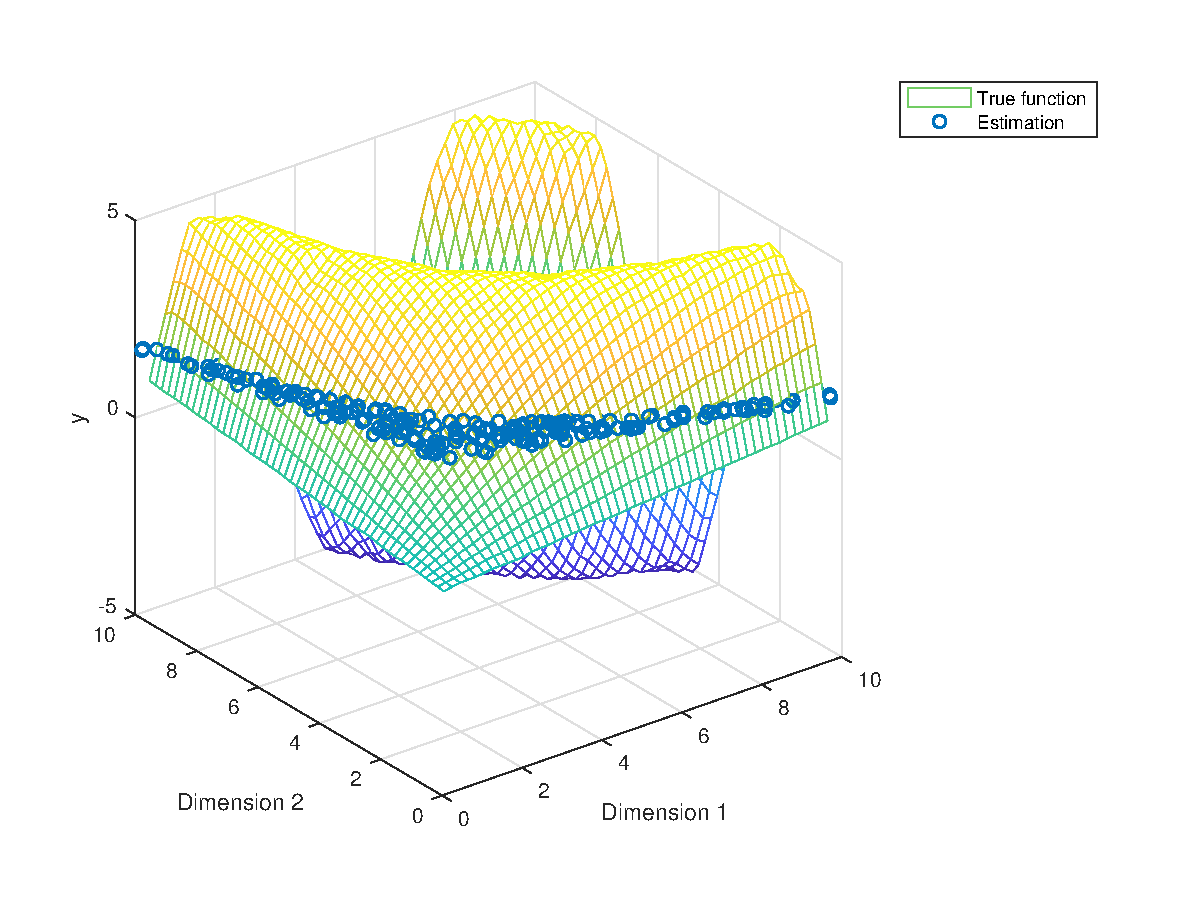
\includegraphics[width=0.8\textwidth]{project41c2}
\end{figure}

\subsubsection{Polynomial models}
\begin{table}[H]
	\centering
	\caption{Mean square error}
	\label{tab:twodimData}
	\begin{tabular}{@{}ccccc@{}}
		\toprule
		Polynomial degree & 2   & 3   & 4   & 5   \\ \midrule
		twoDimData1       & 0.1 & 0.2 & 0.3 & 0.4 \\
		twoDimData2       & 8.5 & 5.0 & 4.2 & 2.9 \\ \bottomrule
	\end{tabular}
\end{table}

\subsubsection{KNN model}

\textbf{twoDimData1}: Given 100 generated data, the KNN model gives the best estimation result when choosing the number of neighbors around $K=10$, and the polynomial model outperforms the KNN. Increasing the number of data will not change the comparison result. However, when the data size is very small, e.g., 10, both the polynomial model and the KNN cannot provide a good estimation. In this case, which model is better depends on the stochastically generated data.

\textbf{twoDimData2}: Given 100 generated data, the KNN model gives the best estimation result when choosing the number of neighbors around $K=3$, and the KNN outperforms the polynomial model. Empirical results show that increasing or decreasing the number of data may influence the optimal number of neighbors but will not change the comparison result.

\subsection{Ten dimensional data} 

\subsubsection{Number of regressors}
Given a ten dimensional data, a linear regression model has 11 regressors, one for constant, and ten for linear terms. For a linear regression model containing polynomial regressors up to degree 3, it has 1 regressor for constant term, ${10}\choose{1}$ regressors for linear term, ${{10}\choose{1}}+{{10}\choose{2}}$ regressors for quadratic term and ${{10}\choose{1}}+2{{10}\choose{2}}+{{10}\choose{3}}$ for cubic term (in total 286 regressors). 

\subsubsection{Testing result of linear regression model}
A linear regression model outperforms a polynomial model with degree 3 without regularization. Adding regularization to the polynomial model can improve the estimation performance substantially. 

\subsubsection{Testing result of KNN}

Empirical results show that, given 1000 data, choosing number of neighbors around $K=30$ gives the best result, and the linear regression with polynomial degree 3 and regularization parameter $\lambda=10$ outperforms the KNN. Increasing the data size will not change the comparison result. However, we found that, when the data size decreases to 500, KNN and linear regression start to have similar performance, and that, if we further decrease the data size, KNN will instead outperform linear regression.

\textbf{Analysis}:  As a general rule, linear regression will tend to outperform KNN when there is a small number of observations per predictor. This rule especially holds for high-dimensional data since the KNN suffers from the curse of dimensionality. However, our observation obeys this general rule. In the regression, we use all the possible regressors up to degree 3 to fit the model. However, it is more often the case that the response is only related to a subset of the regressors. In order to fit a single model involving regressors that are associated with the response, variable selection should have been done. Using redundant regressors will increase the chance to fit unexpected pattern in the data that are randomly generated by noise; thus estimation performance might be deteriorated. This explains our observation that the KNN outperforms the linear regression model when the data size is small. 






\end{document}
